\chapter{Knowledge-Based System Extraction from Deep Learning Models}
\label{chap:kbsextractiondl}
%ENLAZAR ESTO CON LOS PRINCIPIOS DE EXPLICABILIDAD DE PHILLIPS ET AL..
\blfootnote{Elvira Amador-Domínguez, Emilio Serrano, & Daniel Manrique (2021). A hierarchical multi-agent architecture based on virtual identities to explain black-box personalization policies. Expert Syst. Appl., 186, 115731. doi:10.1016/j.eswa.2021.115731

}
\section{Knowledge Extraction from Deep Learning Models}
In this context, the DL model acts as a passive element, from which KBS is extracted by means of a middleware model. Method design parameters for KBS extraction from DL models are depicted in Figure \ref{fig:kbs_extra_dl_overview}.
\begin{figure}[t]
    \centering
    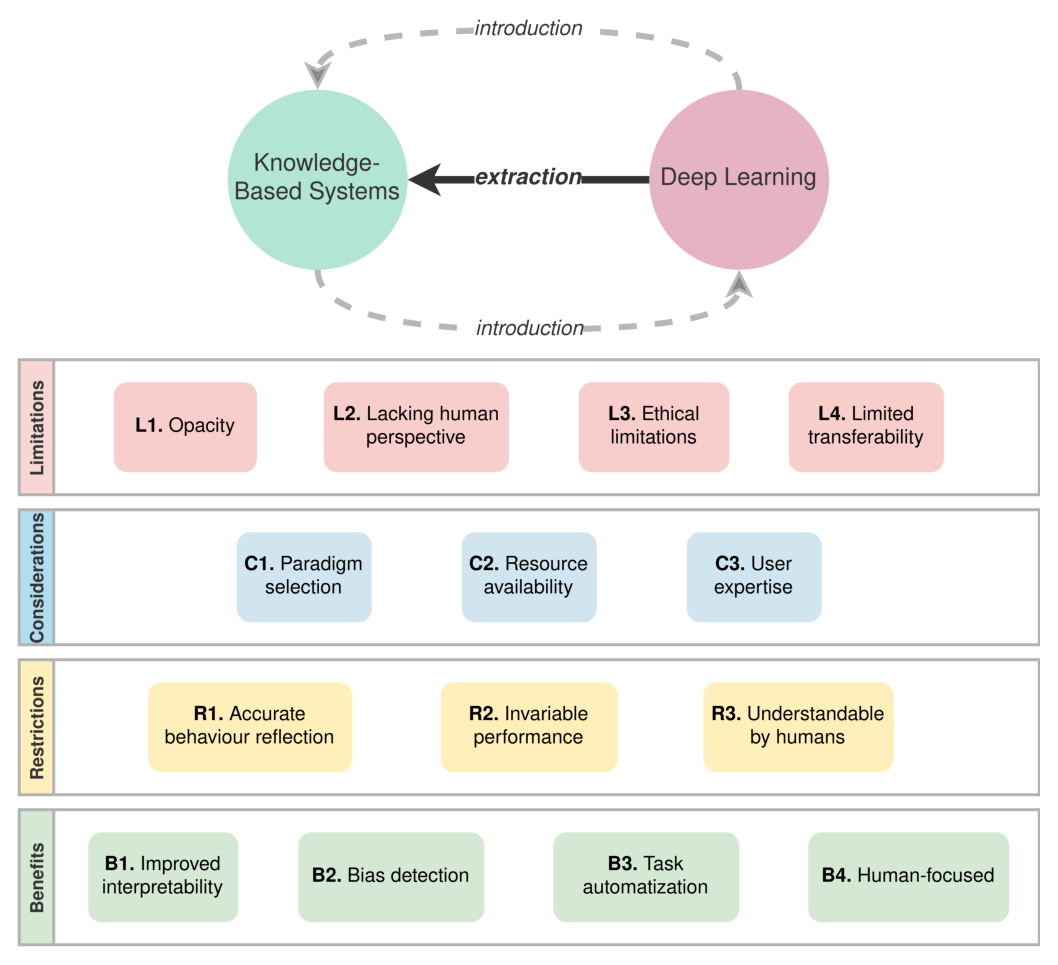
\includegraphics[width=\linewidth]{6_kbsextractiondl/figures/K_extraction_DL.eps}
    \caption{Overview on the Extraction of Knowledge-Based Systems from Deep Learning Models}
    \label{fig:kbs_extra_dl_overview}
\end{figure}

\subsection{Limitations}
\begin{enumerate} [start=1,label={\bfseries L\arabic*.}]
    \item \textbf{Opacity.} \label{kbsextradl_L_opacity} As outlined in the limitations of KBS insertion in DL (Section \ref{4_sec:methodology_kbs_intro_dl}, \ref{kbsintrodl_L_opacity}), opacity is one of the main drawbacks of DL models. While some recent efforts aim to provide an insight on the inference process followed by a DL model to generate a certain output from a given input, these insights are only approximated. Therefore, explainations can reliably capture the behaviour of the DL model, but it cannot be fully ascertain that they are an accurate depiction of the DL model's internal behaviour.

    \item \textbf{Lacking human perspective.} \label{kbsextradl_L_human} DL models are devised to operate autonomously, without the need of human intervention. This phenomenon may be beneficial in some scenarios, but it may be detrimental in those scenarios where user perspective is important. Such is the case of health related scenarios, where only expert users make final decisions, as DL model predictions may not be fully trusted or justified. 
    
    \item \textbf{Ethical limitations.} \label{kbsextradl_L_ethical} DL models infer patterns entirely from training data. Therefore, the inferred patterns are not subject to any ethical considerations. This issue is particularly concerning, as biases within the data can lead to the inference of patterns that may be discriminating or exhibit some ethical concerns.
    
    \item \textbf{Limited transferability.}\label{kbsextradl_L_transferability} The lack of understanding on the internal behaviour of DL models not only conditions its interactions with users, but also between models. This hinders the transferability of DL models, as it can not be ascertain beforehand how a model will behave on a different scenario.
\end{enumerate}

\subsection{Considerations}
\begin{enumerate} [start=1,label={\bfseries C\arabic*.}]
    \item \textbf{Paradigm selection.} \label{kbsextradl_C_paradigm} KBS extraction from DL usually requires from one or more middleware models that perform the extraction and the conversion. Therefore, these models must be aligned with both the final KBS and the initial DL model. Moreover, if the KBS is devised as an explanatory mean for the DL model, it is also key to select a type of KBS that can accurately depict its behaviour.
    
    \item \textbf{Resource availability.} \label{kbsextradl_C_resource} As evidenced in the previous interactions, the inclusion of DL models generally carries an additional computational cost. In this scenario, where the DL model is a passive element, its computational cost may not be as remarkable. However, the introduction of middleware models may increase the resource demand. Providing the involved models with sufficient computational resources is therefore essential.
    
    \item \textbf{User expertise.} \label{kbsextradl_C_user} In explainability, the user replaces the DL model as the central element. Therefore, the extracted KBS should not only be aligned with the DL model, but also should be aligned with the final user. User expertise is an essential element in this scenario, as it conditions the KBS selection and behaviour.
\end{enumerate}

\subsection{Restrictions}
\begin{enumerate} [start=1,label={\bfseries R\arabic*.}]
    \item \textbf{Accurate behaviour reflection.} \label{kbsextradl_R_behaviour} If the KBS serves explainatory purposes, then it must be an accurate reflection of the behaviour of the DL model. This implies that the KBS should not be considered a replacement for the DL model, nor improve its performance. The KBS must therefore imitate the behaviour of the DL model, which entails that the predictions of both models (correct and incorrect) must be similar.
    
    \item \textbf{Invariable performance.} \label{kbsextradl_R_performance} As previously described, the DL model plays a passive role in this interaction.  Whether the DL model serves as a source for KBS extraction, or acts as a black-box element to be explained, its performance must remain invariant and unaffected. This is particularly important regarding explainability, as modifications in the DL model may compromise their integrity, leading to inaccurate insights on its behaviour. 
    
    \item \textbf{Human-understandable.} \label{kbsextradl_R_human} KBS are inherently symbolic, producing outputs that are human-readable. However, as denoted in \ref{kbsextradl_C_user}, the understability of the output does not only depend on the model, but on the expertise of the final user. Therefore, KBS must not only be readable, but understandable by humans.
\end{enumerate}

\subsection{Benefits}
\begin{enumerate} [start=1,label={\bfseries B\arabic*.}]
    \item \textbf{Improved interpretability.}\label{kbsextradl_B_interpretability} Opacity is one of the main hardships regarding DL models (\ref{kbsextradl_L_opacity}). Gaining knowledge on the inference process of DL models increases the trust that users may have on the model (\ref{kbsextradl_L_human}). Moreover, it can serve as a scaffold for improving the transferability of the model (\ref{kbsextradl_L_transferability}).
    
    \item \textbf{Bias detection.}\label{kbsextradl_B_bias} Inference patterns learned by DL models are solely based on the input training data. Data is subject to errors, and biases, which may cause the model to learn inferential patterns that, while accurate from a computational standpoint, may not be ethically correct (\ref{kbsextradl_L_ethical}). Becoming aware on the basis on which inference is performed may enable the detection of biases within the data, which can then be corrected.
    
    \item \textbf{Task automatization.}\label{kbsextradl_B_automatization} In addition to the explainability perspective, KBS extraction from DL can also be treated as a means for automatizing several tasks. In Section \ref{sec:sota_knowledge_extraction_dl}, ontology learning was presented as one of these cases, where ontologies were automatically mined. This approach can be taken for the automatization of different tasks, reducing the human effort required to perform them (\ref{kbsextradl_L_human}).
    
    \item \textbf{Human-focused.}\label{kbsextradl_B_human} DL models work virtually autonomously, minimizing the implication of users within the process. Making the models understandable by humans can increase the active implications of users within the learning process not only increasing their trust, but also enhancing the performance of the model from the inclusion of human knowledge (\ref{kbsextradl_L_human}). 
\end{enumerate}
%%HAY DOS CASOS DE USO. DAME TU FUERZA PEGASO QUE SE VIENE LA MADRE DE TODOS LOS INVENTS. 

\section{Summary}